\documentclass[12pt]{report}

\usepackage{geometry}
\usepackage{tabu}
\usepackage{dirtytalk}
\usepackage{graphicx}
\usepackage{url}
\usepackage{float}
\usepackage{listings}
\usepackage{algpseudocode}
\usepackage{algorithm}
\usepackage{algorithmicx}
\usepackage{subcaption}
\usepackage{verbatim}
\usepackage{amsmath}
\usepackage{wrapfig}
\usepackage{color}

\usepackage{amsthm}
\usepackage{verbatimbox}
\usepackage{multicol}
\usepackage[titletoc,title]{appendix}
\usepackage{amsfonts}
\usepackage[font={it}]{caption}
\usepackage{afterpage}
\usepackage{caption}
\usepackage{lipsum}
\usepackage{csquotes}

\usepackage{lmodern}

% For citing and referencing.
\usepackage{natbib}
\newcommand{\citebu}[1]{\citeauthor{#1} (\citeyear{#1})}
\newcommand{\citediagram}[2]{(\citeauthor{#1} \citeyear{#1}, p.#2)}
\newcommand{\citesoftware}[1]{(\citeauthor{#1} \citeyear{#1})}

\newcommand{\figurewidth}{0.6\textwidth}
\newcommand{\imagewidth}{0.5\textwidth}

\newcommand{\quotebu}[1]
{
  \begin{displayquote}
    \textit{#1}
  \end{displayquote}
}

\geometry{
  a4paper,
  total={170mm,257mm},
  left=30mm,
  right=30mm,
  top=20mm,
  bottom=30mm,
}

\pagenumbering{roman}

\theoremstyle{definition}
\newtheorem{definition}{Definition}[section]

\begin{document}

  \renewcommand{\familydefault}{\sfdefault}
  \fontfamily{lmss}\selectfont

  \begin{titlepage}
    \centering
    {\Huge Bournemouth University\par}
    \vspace{0.5cm}
    {\Large National Centre for Computer Animation\par}
    \vspace{0.5cm}
    {\Large MSc in Computer Animation and Visual Effects\par}
    \vspace{5cm}
    {\huge \bfseries evulkan\par}
    \vspace{0.5cm}
    {\Large \bfseries \textit{A Vulkan Library}\par}
    \vspace{2cm}
    {\Large Eimear Crotty\par}
    % \includegraphics[width=0.15\textwidth]{images/MIT.png}\par\vspace{1cm}
    \vfill
    {\Large August 2020}
  \end{titlepage}

  \chapter*{Abstract}
    Vulkan is a low-level graphics API which aims to provide users with faster
    draw speeds by removing overhead from the driver. The user is expected to
    explicitly provide the details previously generated by the driver. The
    resulting extra code can be difficult to understand and taxing to write
    for beginners, leading to the need for a helper library.

  \chapter*{Acknowledgements}

    \vspace{1cm}
    Jon Macey\\
    Mum, Dad, Rory, Aisling, Aoife, Ellie.\\
    Neil.
    % TODO.

  \chapter*{Dedication}

    %TODO

  \tableofcontents

  \listoffigures

  \chapter{Introduction}
    \pagenumbering{arabic}
    Vulkan \citesoftware{vulkan} is a cross-platform graphics and compute API.
    It aims to provide higher efficiency than other current
    cross-platform APIs, by using the full performance available in today's
    largely-multithreaded machines. Vulkan achieves this by allowing tasks to be
    generated and submitted to the GPU in parallel (multithreaded programming).
    In addition, the API itself is written at a lower-level than other graphics
    APIs, meaning that the developer is required to provide many of the details
    previously generated by the driver at run-time.\\

    This project aims to alleviate this cost by providing a wrapper library for
    Vulkan, which allows a developer to use some of the more common features of
    Vulkan with much less effort than writing an application from scratch. This
    library is written in C++, using modern C++ features, adheres to both the
    official C++ Core Guidelines and Google C++ Style Guide and is fully unit
    tested. The library is available for download from GitHub and can be built
    using CMake.\\

    The library is specifically written with beginners and casual users of
    Vulkan in mind. The examples included in the repository provide a
    demonstration of how to use the library for different purposes, including
    drawing a triangle, loading an OBJ with a texture and using multiple passes
    to render simple objects with deferred shading. A non-goal is to create a
    library which is as fast as writing pure Vulkan, however the library
    must be reasonably fast.\\

  \chapter{Previous Work}

    While Vulkan is a relatively new API for graphics and compute, many engines
    now support Vulkan, including CryEngine, Valve's Source, Unity and Unreal
    Engine. As a result, there are many libraries and utilities available
    online for Vulkan, each of which serves a different purpose.

    \section{V-EZ}

      AMD created the open-source V-EZ library \citesoftware{vez}. Its main goal is to increase the
      adoption of Vulkan in the games industry by reducing the complexity of
      Vulkan. It is a lightweight C API wrapped around the basic Vulkan API.
      It is part of the GPU-Open initiative. \\
      
      It still requires the user to have a good knowledge of Vulkan, making it
      difficult for beginners to adopt. For example, some rather complex
      components include semaphores, swapchain creation and lengthy
      enumerations such as

        \begin{figure}[h!]
        \centering
        \verb|VK_BUFFER_USAGE_TRANSFER_DST_BIT|
        \end{figure}

      While it does remove some of the boilerplate, it is still relatively low
      level and, as a result, is not perfectly suited to beginners.

    \section{Anvil}

      The goal of Anvil is to reduce the amount of time taken to write Vulkan
      applications. It is ideal for rapidly prototyping Vulkan applications,
      but it still requires a large amount of writing. It is stated in the
      documentation itself that Anvil is not suitable for beginners.

      \quotebu{
        Anvil is not the right choice for developers who do not have a
        reasonable understanding of how Vulkan works.
      }

  \chapter{Technical Background}
  
    \begin{figure}[h]
      \centering
      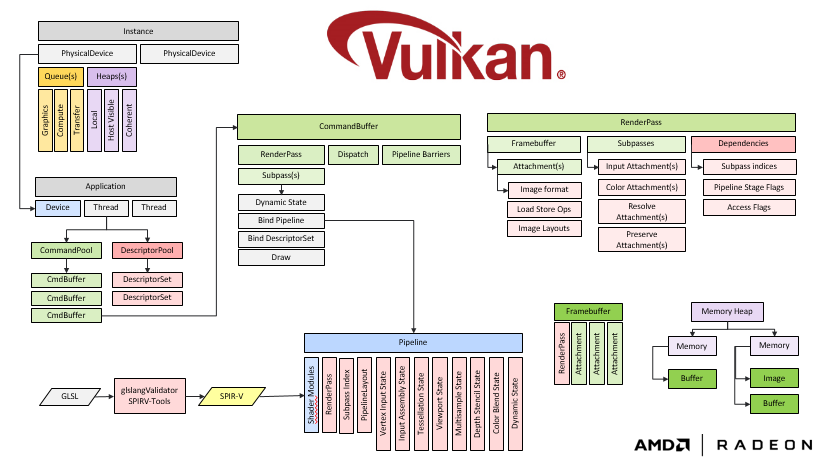
\includegraphics[width=\textwidth]{images/interactions.png}
      \caption{Vulkan API objects and their interactions \citediagram{vez}{1}.}
      \label{fig:interactions}  
    \end{figure}

    \section{Limitations of OpenGL}
    OpenGL, the current cross-platform industry standard, was first released in 1992.

  \chapter{The evulkan Library}

  \lipsum[1]

  \begin{wrapfigure}{l}{\figurewidth}
    \centering
    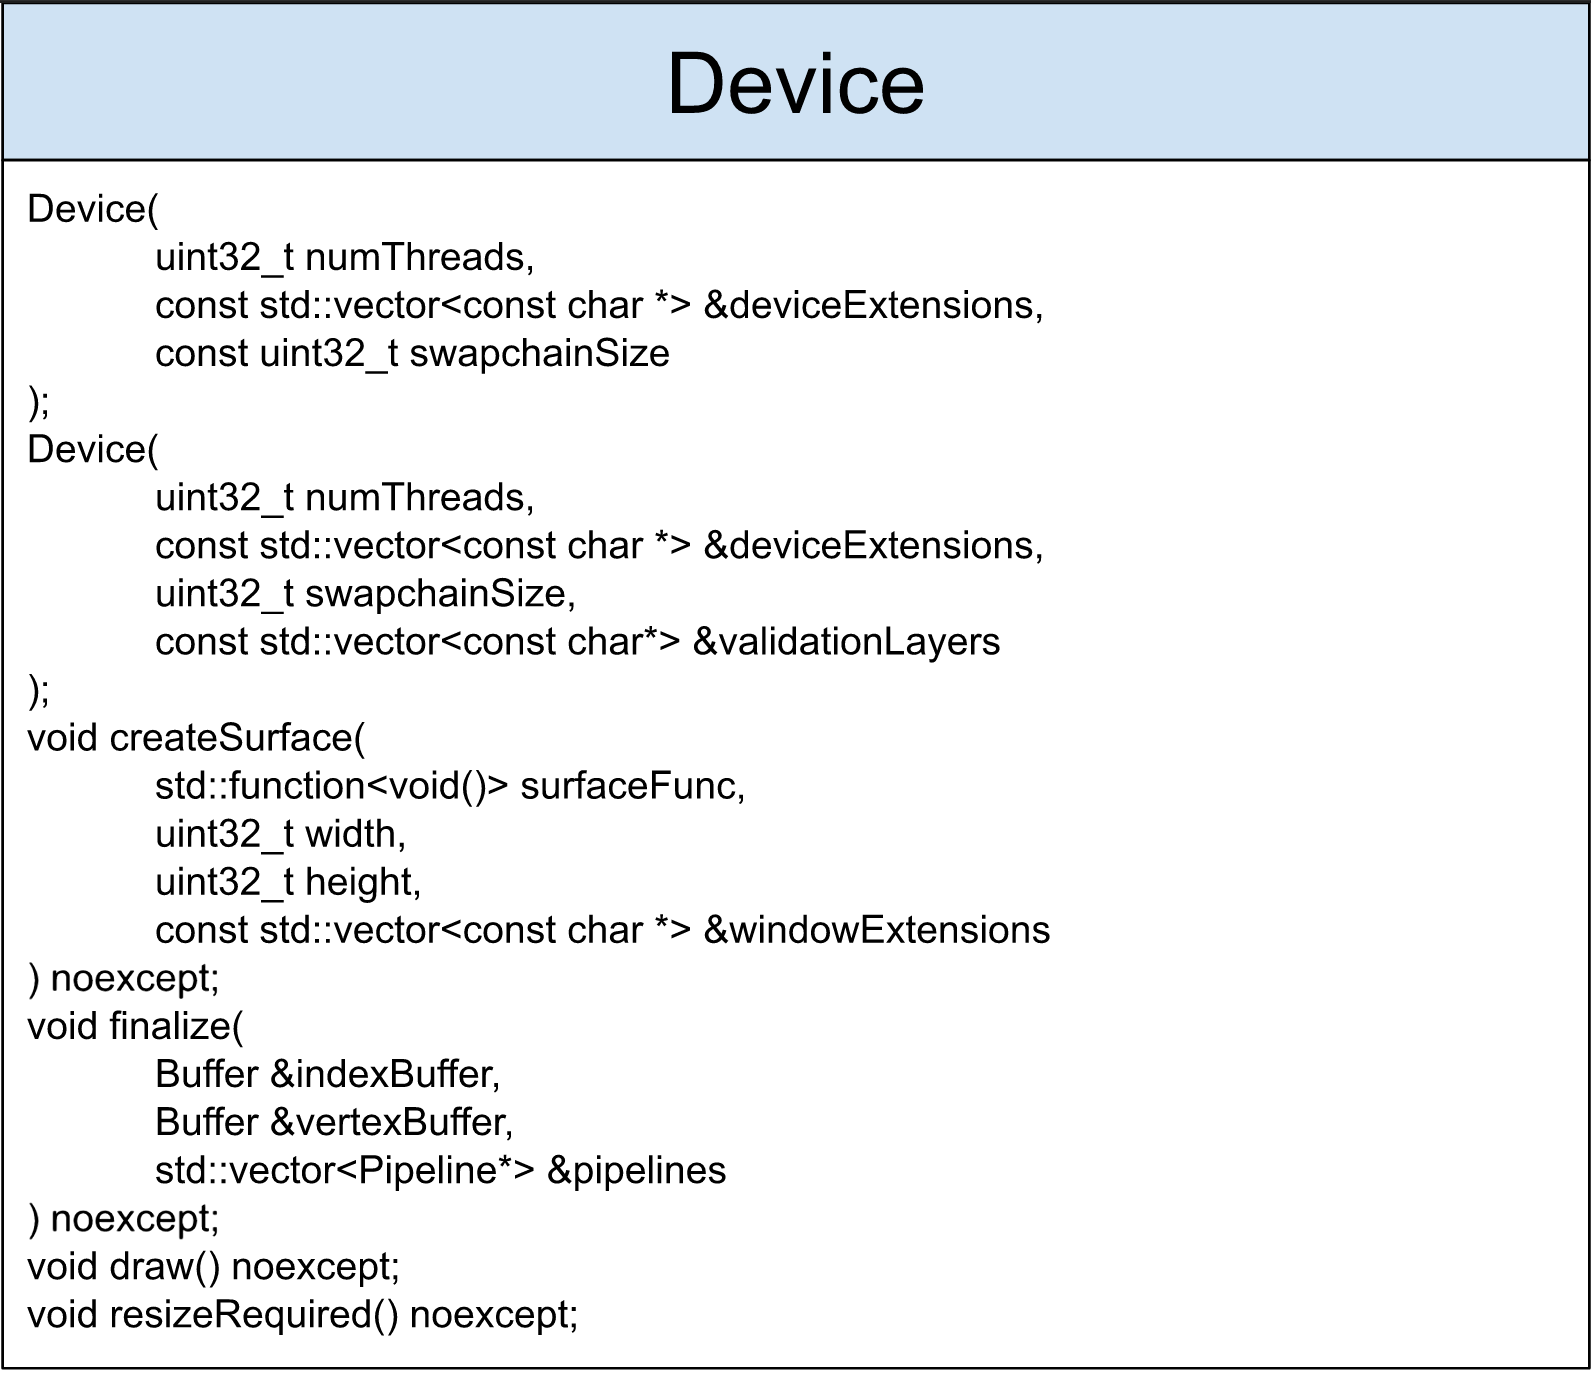
\includegraphics[width=\imagewidth]{images/class_device.png}
    \caption{Device class diagram.}
    \label{fig:class_device}  
  \end{wrapfigure}

  \begin{wrapfigure}{l}{\figurewidth}
    \centering
    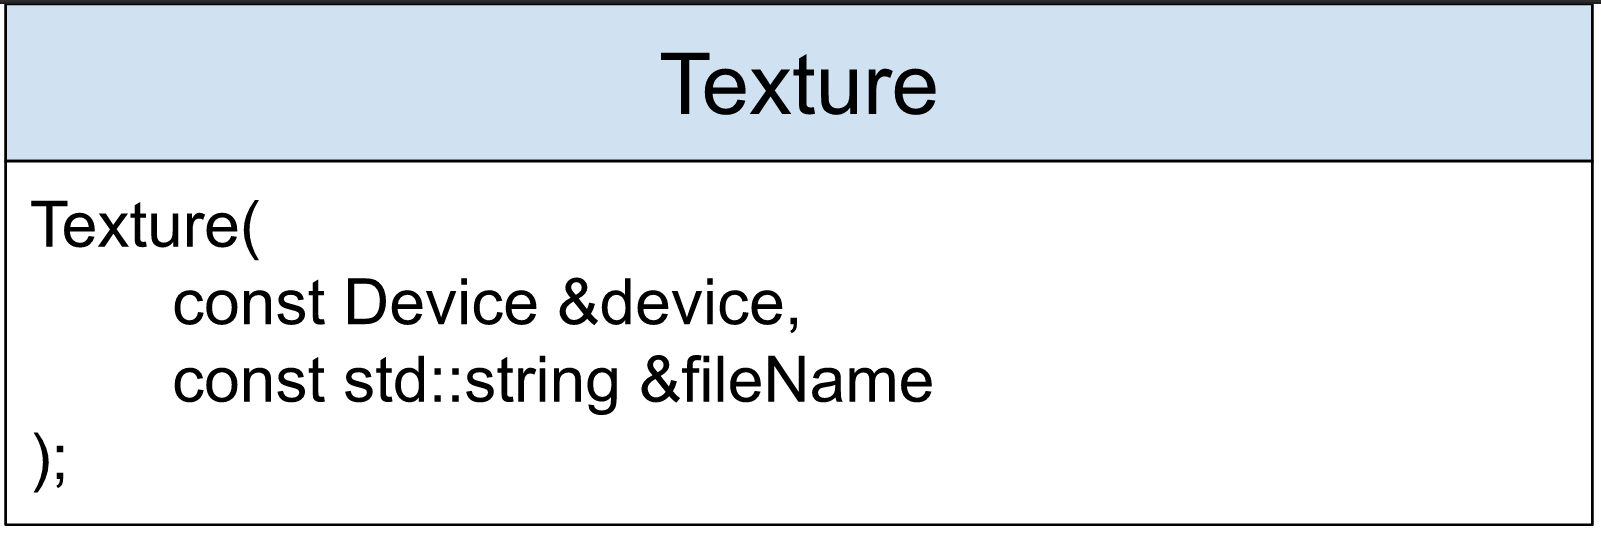
\includegraphics[width=\imagewidth]{images/class_texture.png}
    \caption{Texture class diagram.}
    \label{fig:class_texture}  
  \end{wrapfigure}

  \begin{wrapfigure}{l}{\figurewidth}
    \centering
    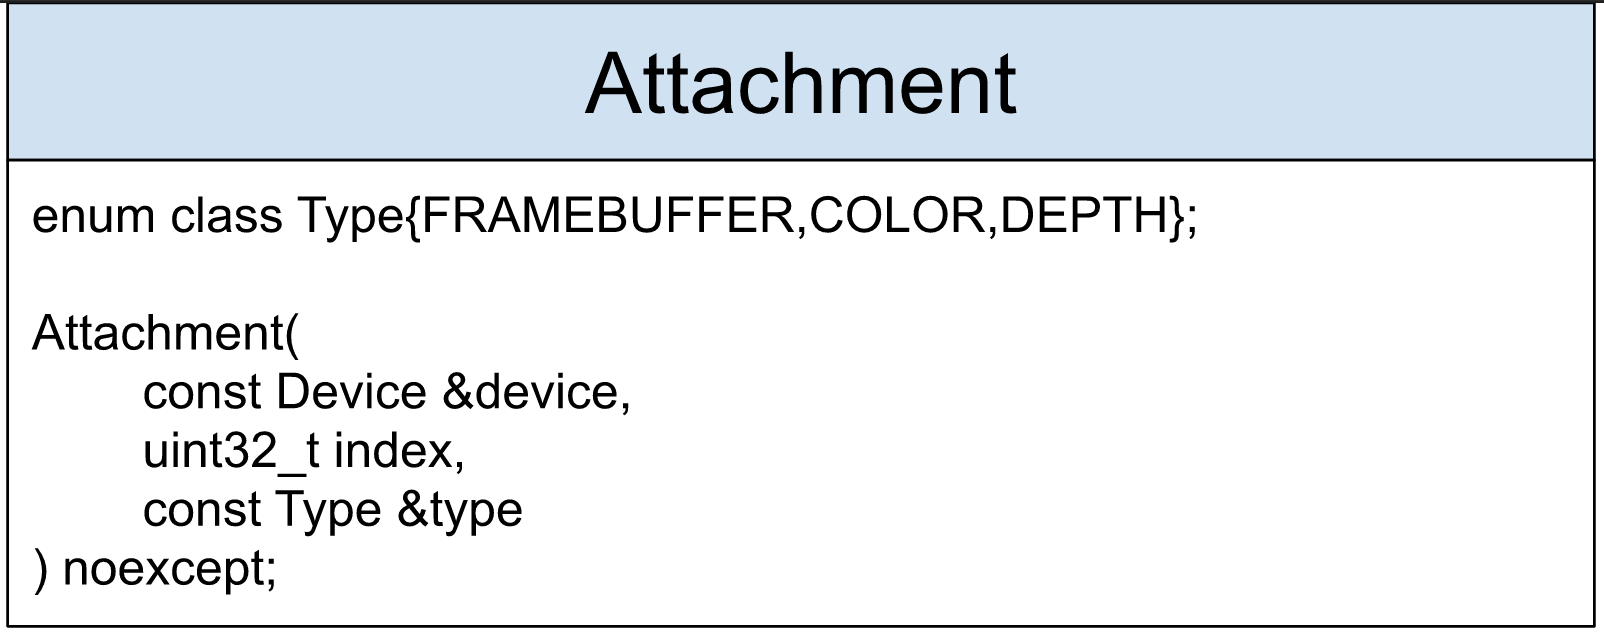
\includegraphics[width=\imagewidth]{images/class_attachment.png}
    \caption{Attachment class diagram.}
    \label{fig:class_attachment}  
  \end{wrapfigure}

  \lipsum[3]

  \begin{wrapfigure}{l}{\figurewidth}
    \centering
    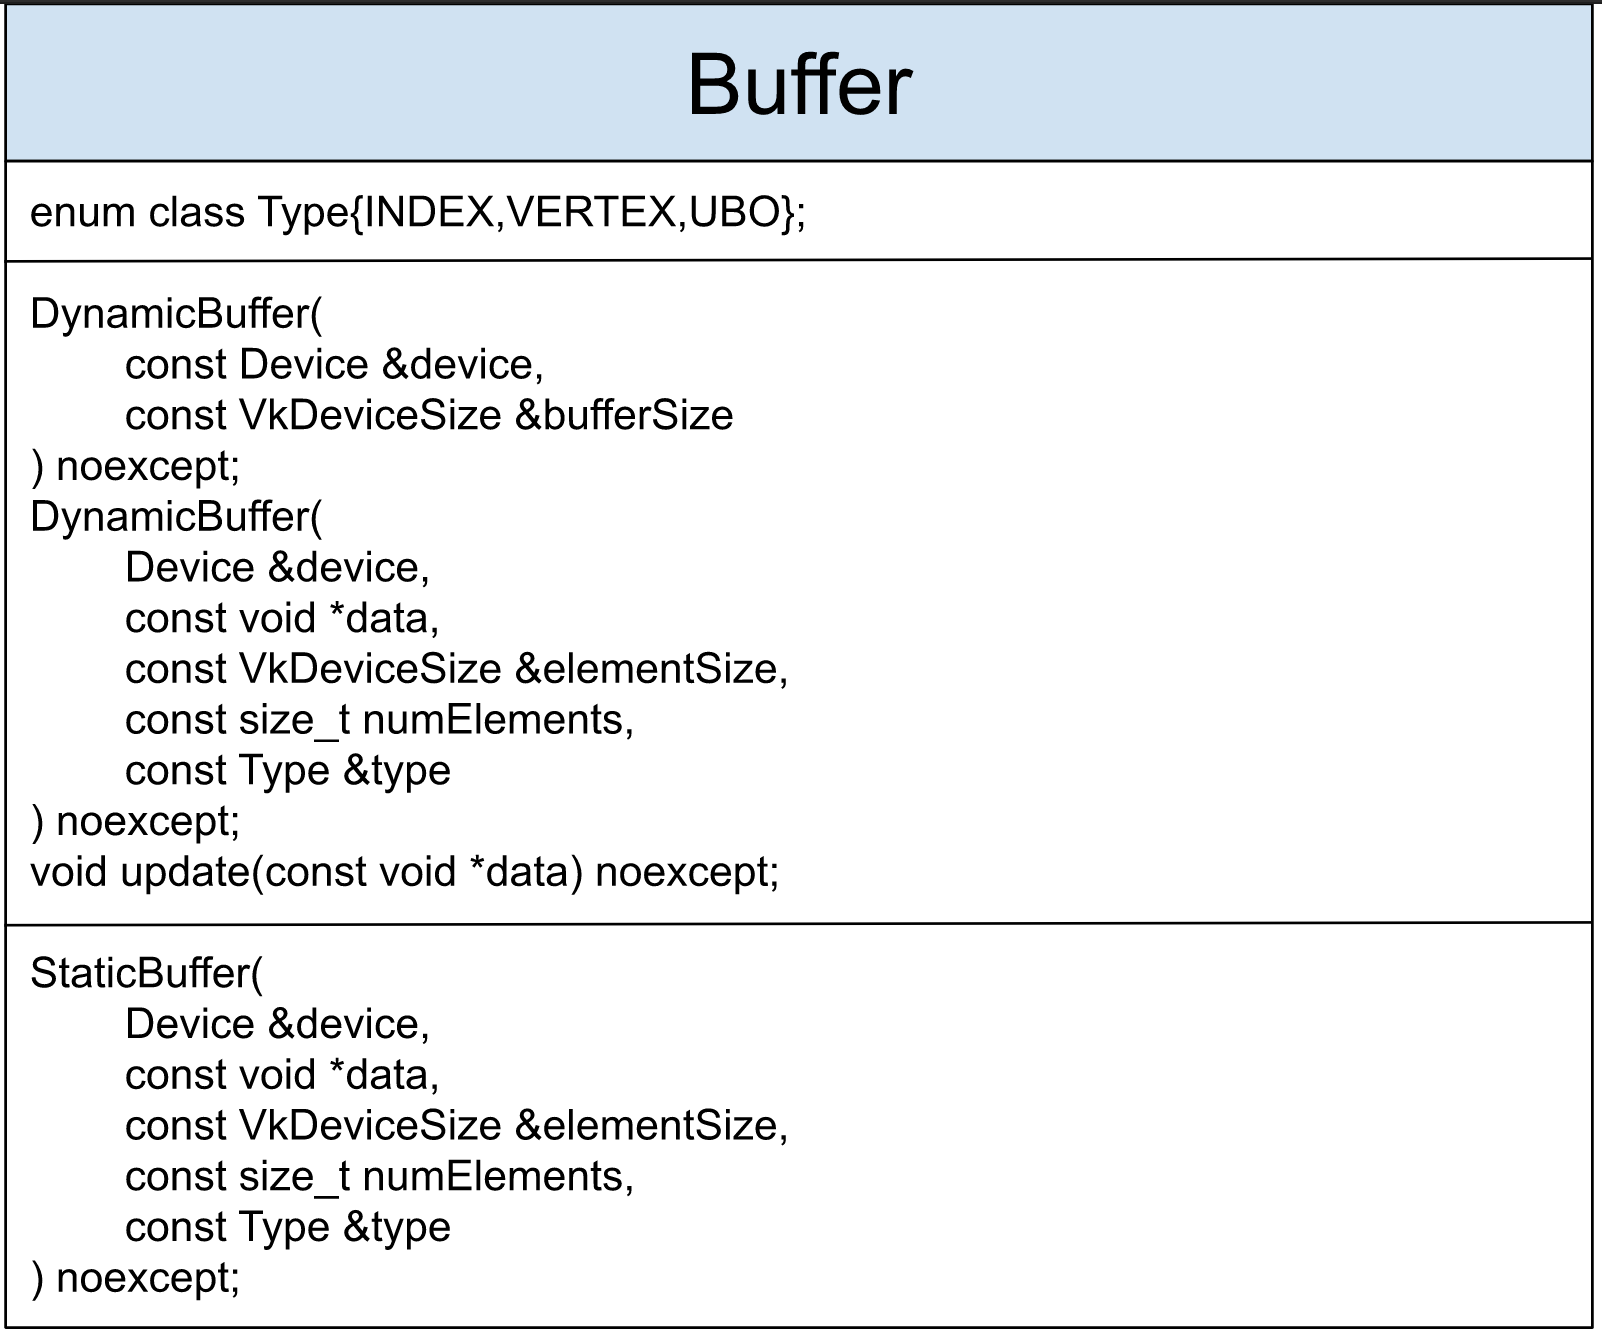
\includegraphics[width=\imagewidth]{images/class_buffer.png}
    \caption{Buffer class diagram.}
    \label{fig:class_buffer}  
  \end{wrapfigure}

  \begin{wrapfigure}{l}{\figurewidth}
    \centering
    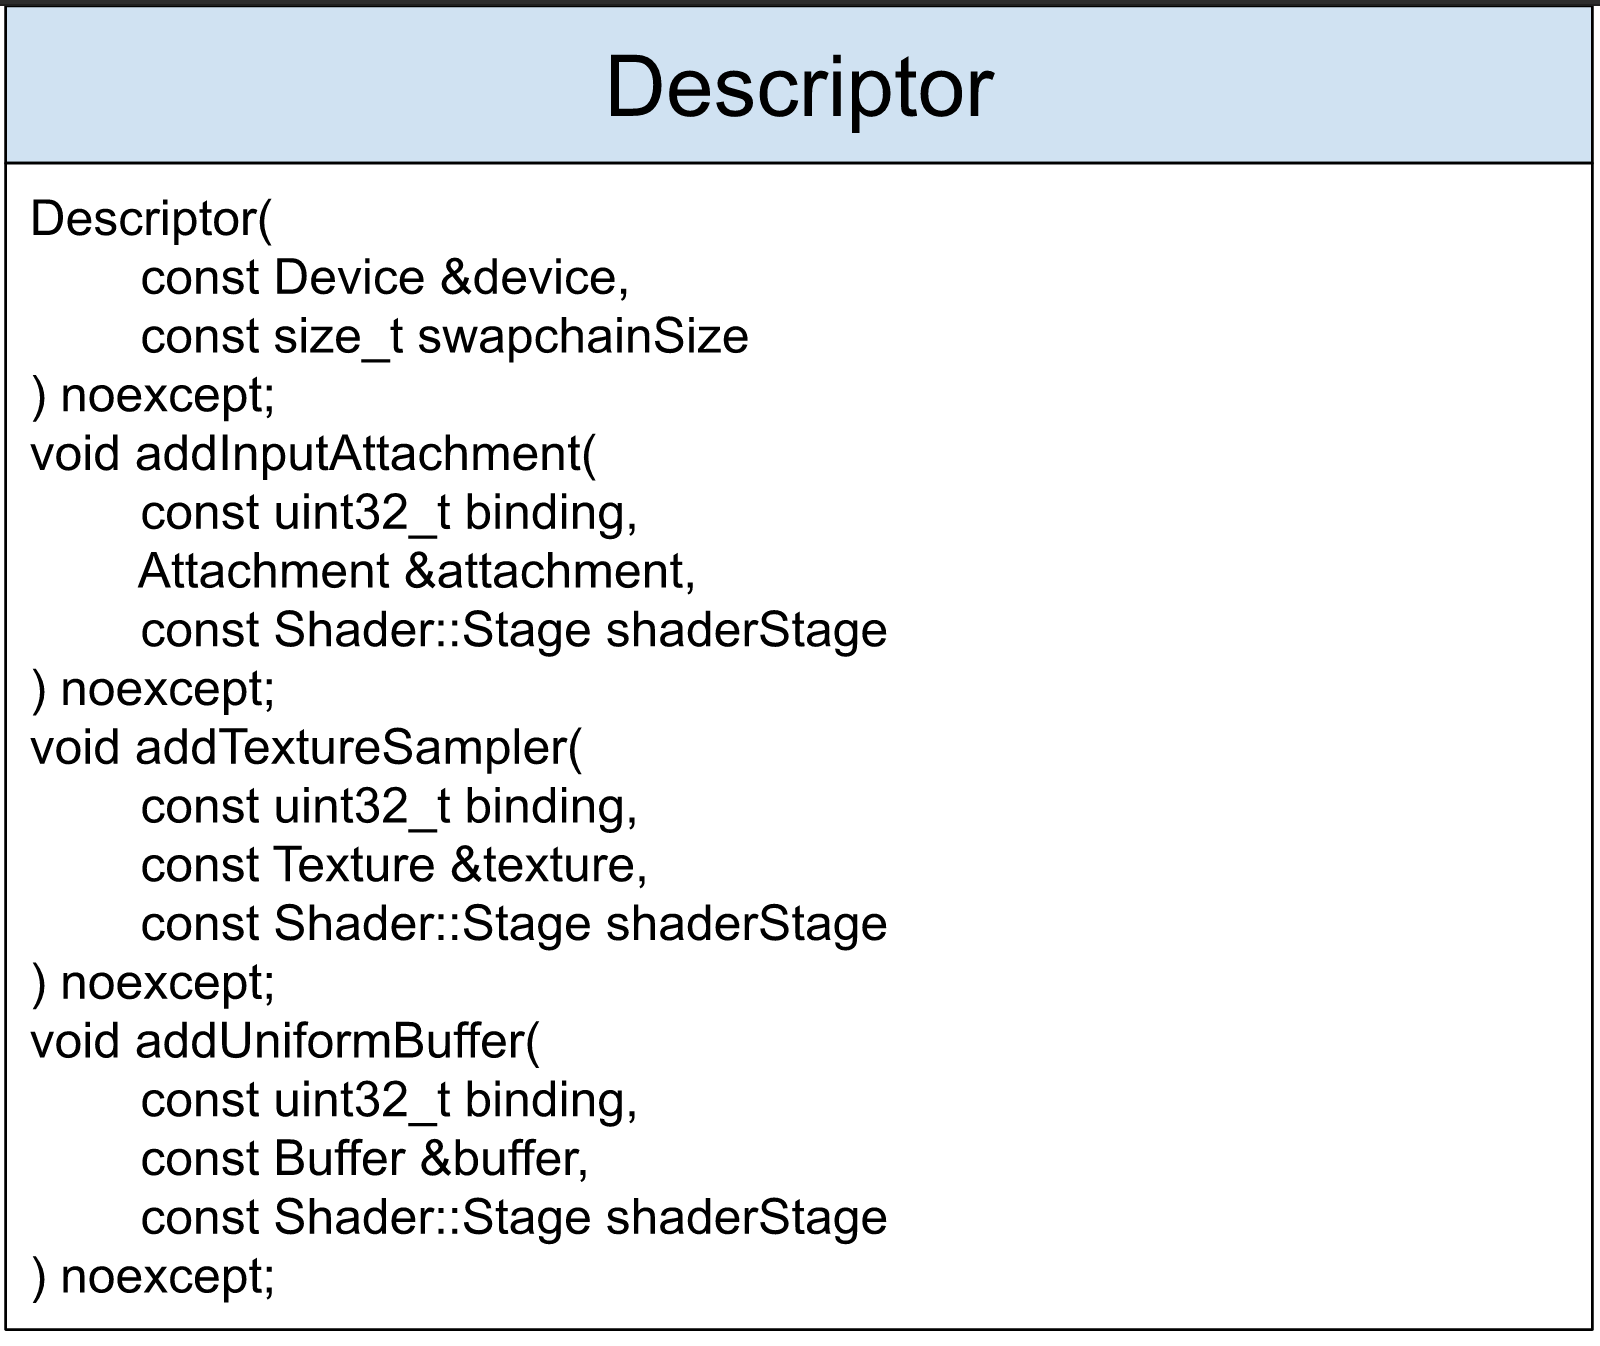
\includegraphics[width=\imagewidth]{images/class_descriptor.png}
    \caption{Descriptor class diagram.}
    \label{fig:class_descriptor}
  \end{wrapfigure}

  \begin{wrapfigure}{l}{\figurewidth}
    \centering
    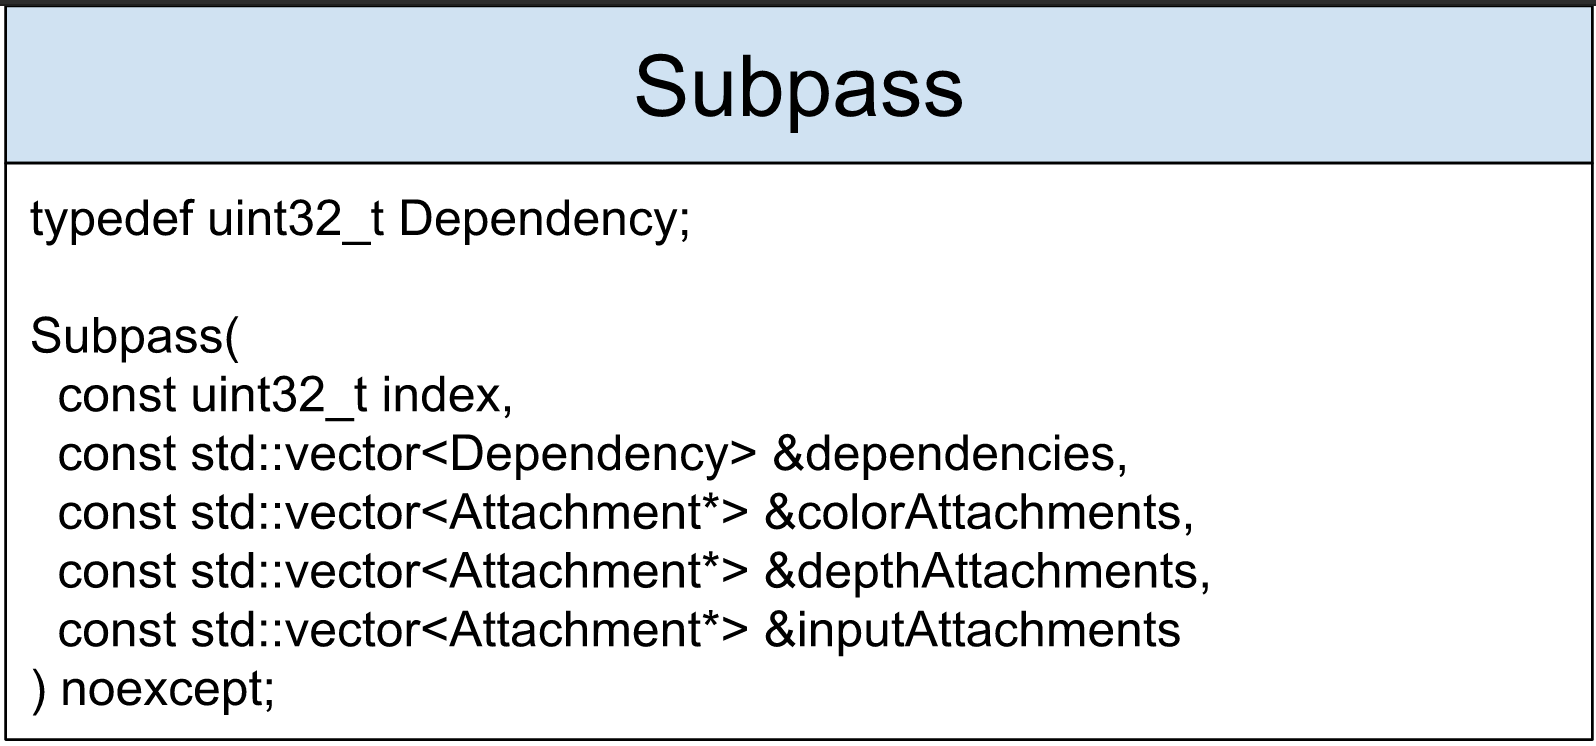
\includegraphics[width=\imagewidth]{images/class_subpass.png}
    \caption{Subpass class diagram.}
    \label{fig:class_subpass}
  \end{wrapfigure}

  \begin{wrapfigure}{l}{\figurewidth}
    \centering
    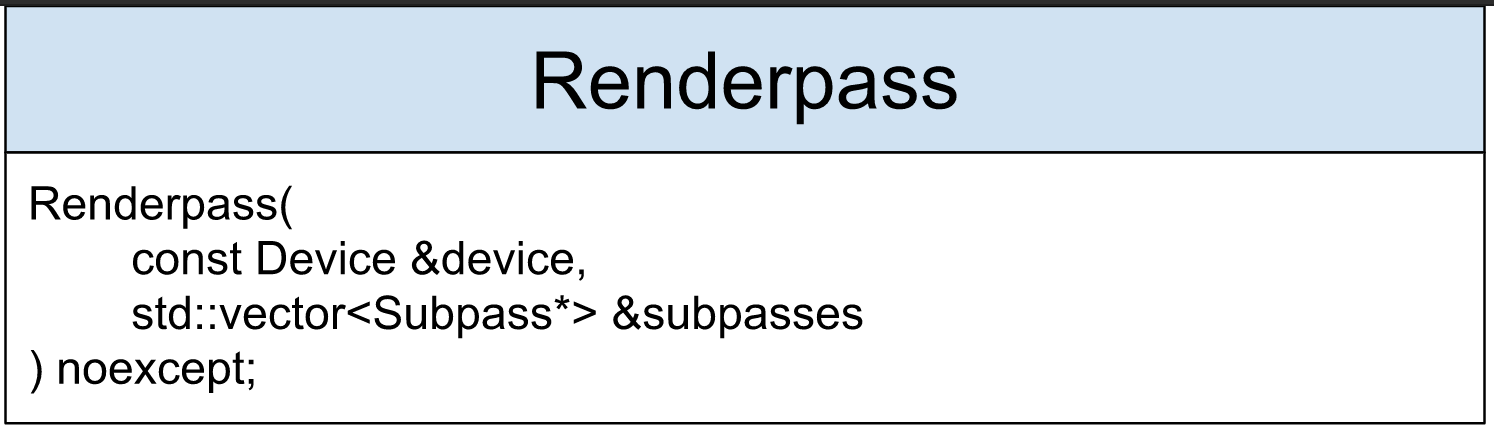
\includegraphics[width=\imagewidth]{images/class_renderpass.png}
    \caption{Renderpass class diagram.}
    \label{fig:class_renderpass}
  \end{wrapfigure}

  \begin{wrapfigure}{l}{\figurewidth}
    \centering
    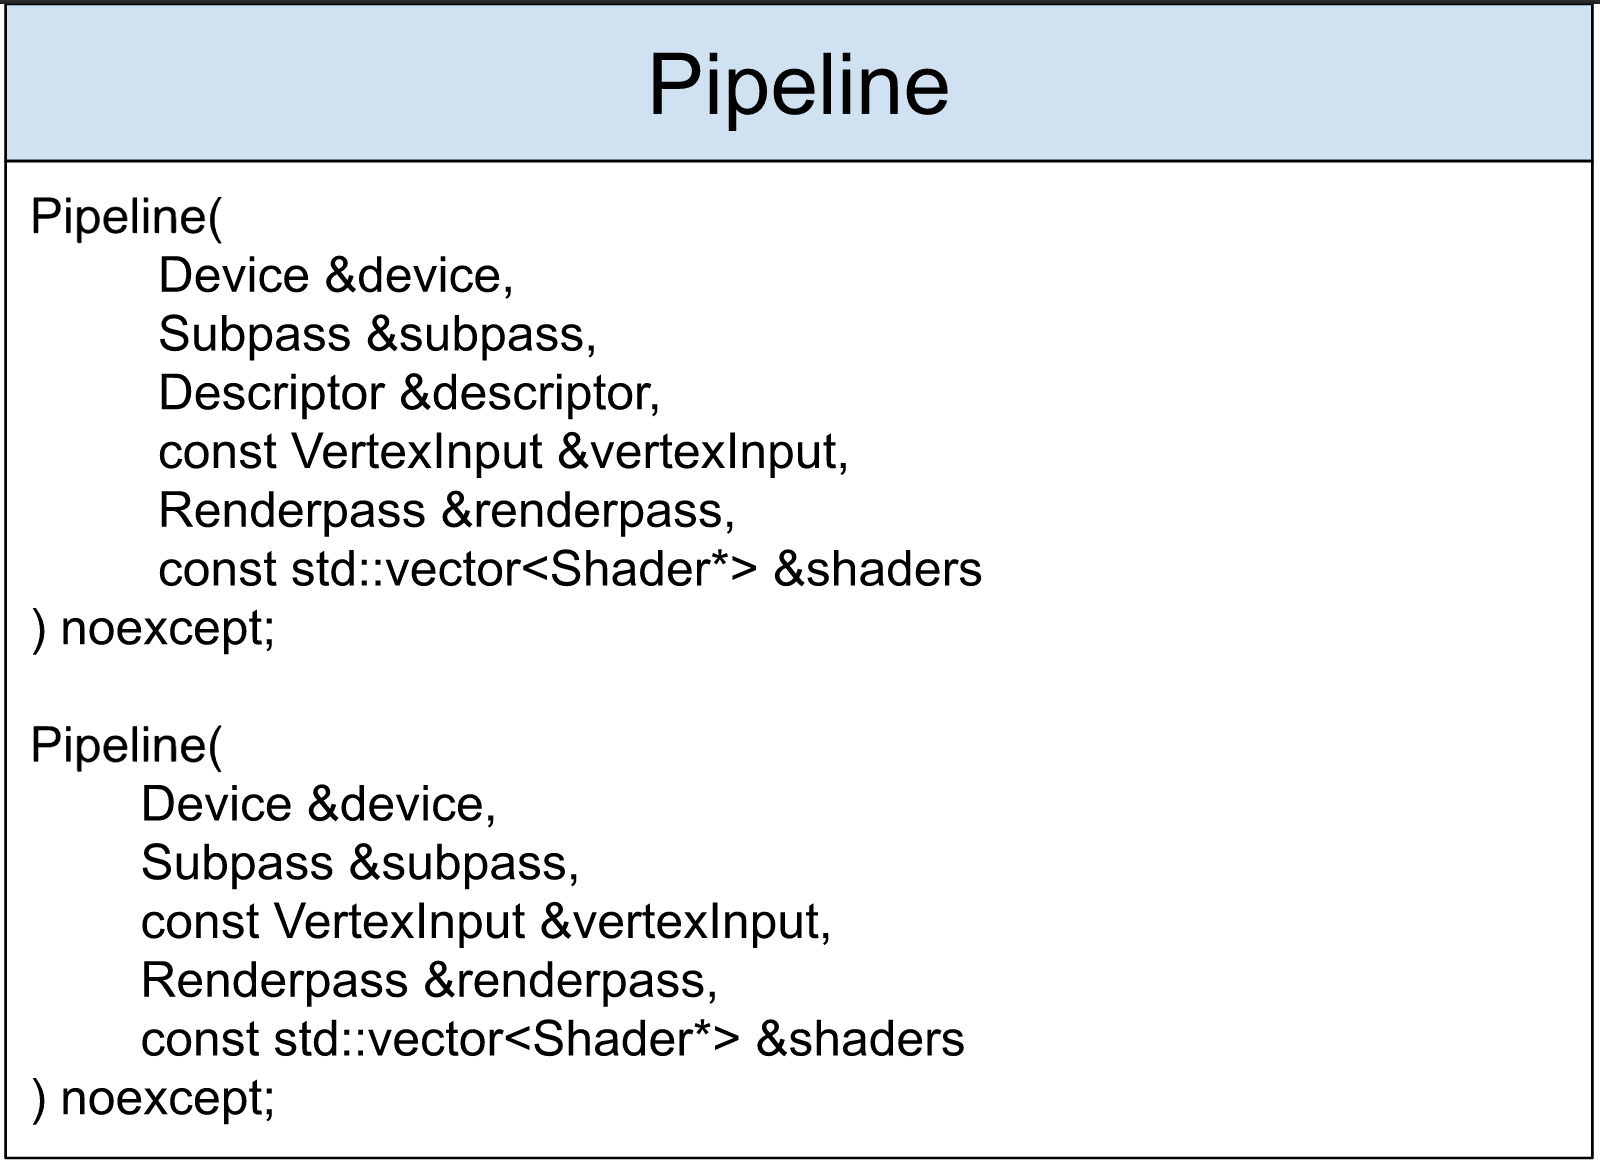
\includegraphics[width=\imagewidth]{images/class_pipeline.png}
    \caption{Pipeline class diagram.}
    \label{fig:class_pipeline}
  \end{wrapfigure}

  \begin{wrapfigure}{l}{\figurewidth}
    \centering
    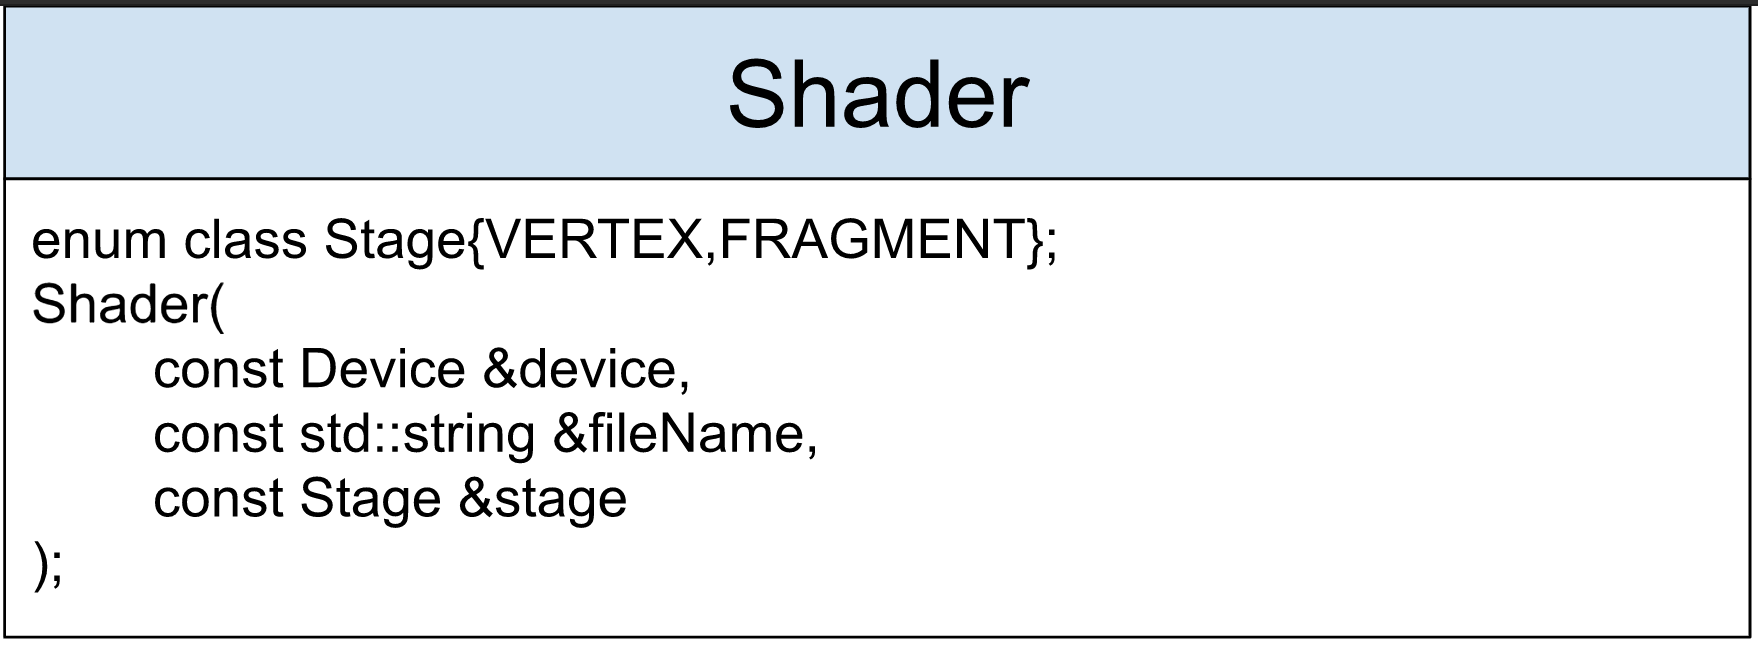
\includegraphics[width=\imagewidth]{images/class_shader.png}
    \caption{Shader class diagram.}
    \label{fig:class_shader}
  \end{wrapfigure}

  \begin{wrapfigure}{l}{\figurewidth}
    \centering
    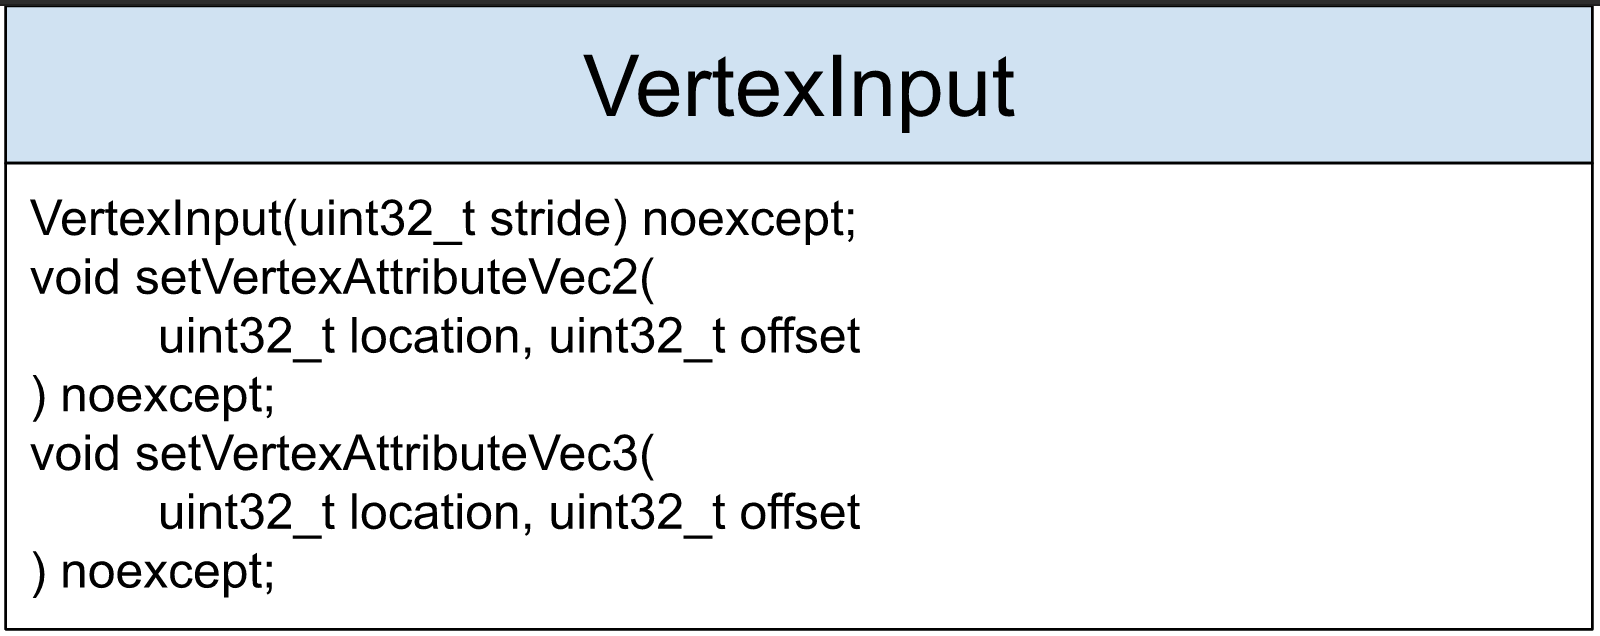
\includegraphics[width=\imagewidth]{images/class_vertexinput.png}
    \caption{VertexInput class diagram.}
    \label{fig:class_vertexinput}
  \end{wrapfigure}

  \chapter{Conclusion}

  \afterpage
  {
    \begin{figure}
      \begin{subfigure}[b]{\textwidth}
        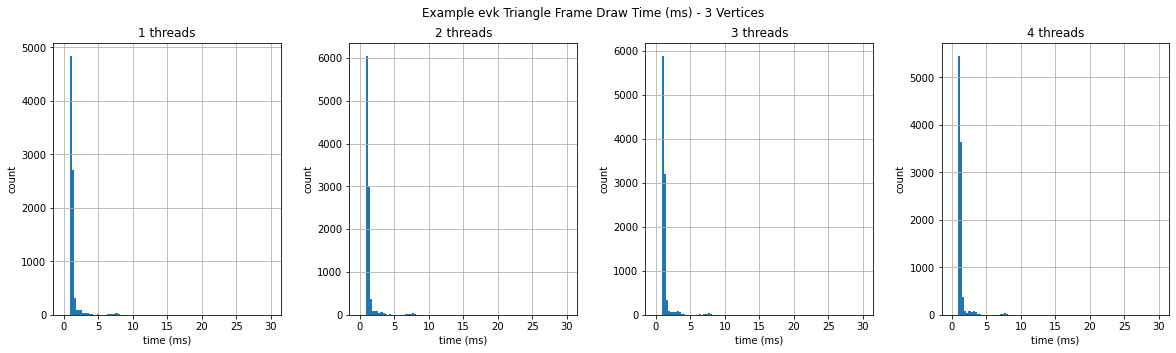
\includegraphics[width=\textwidth]{images/triangle_draw.png}
      \end{subfigure}
      \begin{subfigure}[b]{\textwidth}
        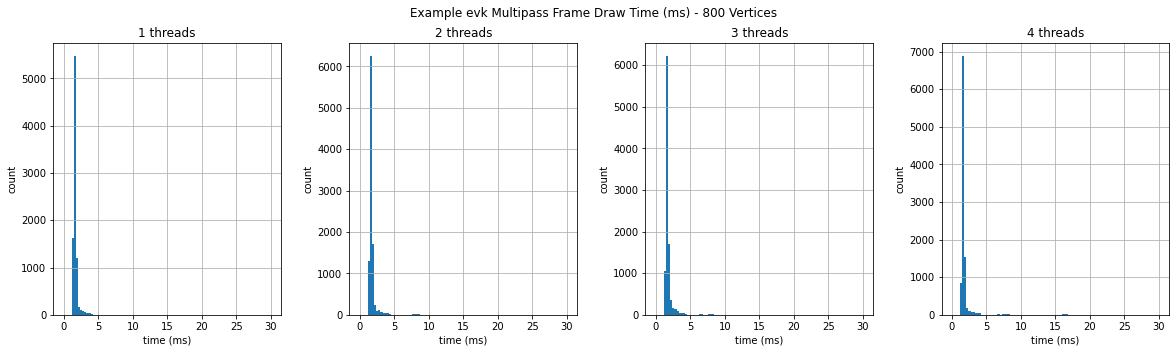
\includegraphics[width=\textwidth]{images/multipass_draw.png}
      \end{subfigure}
      \begin{subfigure}[b]{\textwidth}
        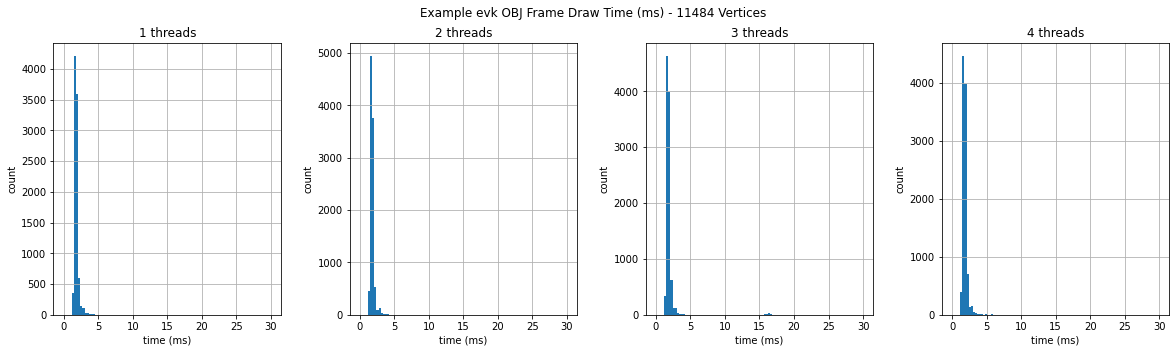
\includegraphics[width=\textwidth]{images/obj_draw.png}
      \end{subfigure}
      \caption{Draw time for different examples over multiple threads.}
      \label{fig:draw}                        
    \end{figure}

    \clearpage

    \begin{figure}
      \begin{subfigure}[b]{\textwidth}
        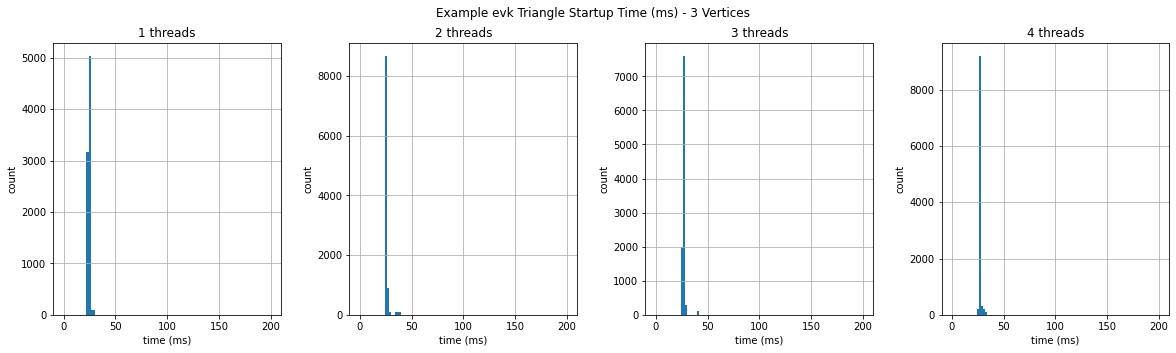
\includegraphics[width=\textwidth]{images/triangle_setup.png}
      \end{subfigure}
      \begin{subfigure}[b]{\textwidth}
        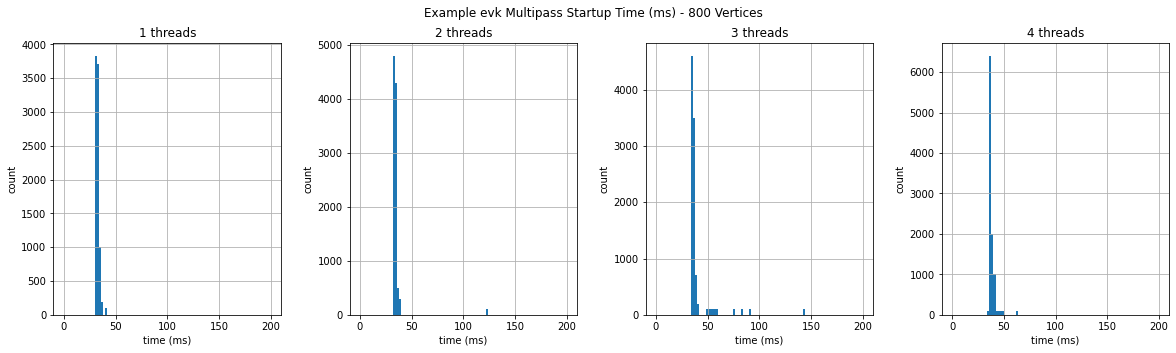
\includegraphics[width=\textwidth]{images/multipass_setup.png}
      \end{subfigure}
      \begin{subfigure}[b]{\textwidth}
        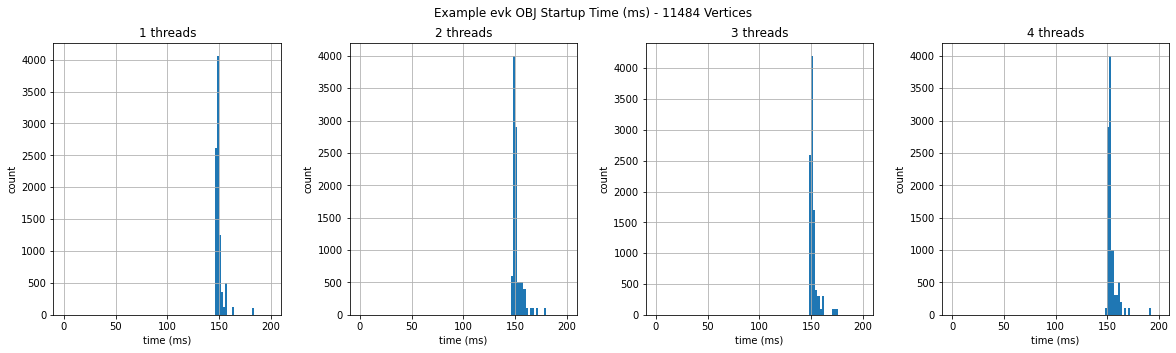
\includegraphics[width=\textwidth]{images/obj_setup.png}
      \end{subfigure}
      \caption{Setup time for different examples over multiple threads.}
      \label{fig:setup}                        
    \end{figure}
    
    \clearpage
  }

  \bibliographystyle{harvardnat}
  \bibliography{thesis.bib}

  \chapter*{Appendices}
  
\end{document}